\documentclass[tikz]{standalone}

\usepackage[T1]{fontenc}
\usepackage[utf8]{inputenc}
\usepackage{eulervm}
\usepackage{amsmath}
\usepackage{bm}
\usepackage{tikz}
\usepackage{environ}

\usetikzlibrary{fit}
\usetikzlibrary{patterns}
\usetikzlibrary{arrows}

\input{./settings/colors}

\begin{document}
  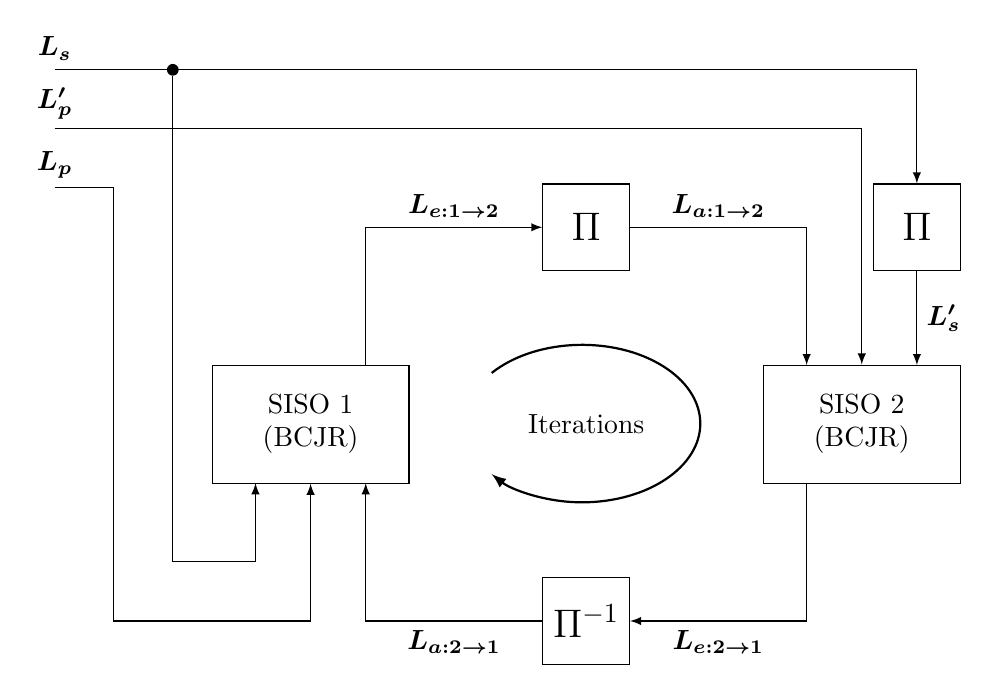
\begin{tikzpicture}%[scale=\tikzscale]
  \tikzset{STA/.style={draw, minimum height=0.65cm, minimum width=0.65cm} }
  \tikzset{SISO/.style={draw, minimum height=1.50cm, minimum width=2.5cm} }
  \tikzset{PI/.style={draw, minimum height=1.10cm, minimum width=1.10cm} }

  \node[SISO, align=center] (siso1) at (0.0, 0.0) {SISO 1\\(BCJR)};
  \node[SISO, align=center] (siso2) at (7.0, 0.0) {SISO 2\\(BCJR)};

  \node[PI, align=center] (pi1) at (7.7, +2.5) {\Large{$\Pi$}};
  \node[PI, align=center] (pi2) at (3.5, +2.5) {\Large{$\Pi$}};
  \node[PI, align=center] (pi3) at (3.5, -2.5) {\Large{$\Pi^{-1}$}};

  \draw[->,>=latex] (pi1.south) -- (7.7,0.75) node [midway, right] {$\bm{L'_s}$};
  \draw[->,>=latex] (pi2.east)  -- (6.3,2.5) node [midway, above] {$\bm{L_{a:1 \rightarrow 2}}$} -- (6.3,0.75);
  \draw[->,>=latex] (6.3,-0.75) -- (6.3,-2.5) -- (pi3.east) node [midway, below] {$\bm{L_{e:2 \rightarrow 1}}$};
  \draw[->,>=latex] (pi3.west)  -- node [midway, below] {$\bm{L_{a:2 \rightarrow 1}}$} (0.7,-2.5) -- (0.7,-0.75);
  \draw[->,>=latex] (0.7,+0.75) -- (0.7,2.5) -- (pi2.west) node [midway, above] {$\bm{L_{e:1 \rightarrow 2}}$};

  \draw[->,>=latex] (-3.25,4.50) node [left, above] {$\bm{L_s}$} -| (pi1);
  \draw[->,>=latex] (-3.25,3.75) node [left, above] {$\bm{L'_p}$} -| (siso2);
  \draw[->,>=latex] (-3.25,3.00) node [left, above] {$\bm{L_p}$} -- (-2.50,3.0) |- (-2,-2.5) -| (siso1.south);

  \node (d0) at (-1.75,4.50) [circle,fill,inner sep=1.5pt]{};

  \draw[->,>=latex] (d0) |- (-0.7,-1.75) -- (-0.7,-0.75);

  \draw [-latex, thick, rotate=+90] (0.65,-2.3) arc [start angle=50, end angle=-230, x radius=1cm, y radius=1.5cm];
  \node at (3.5,0) {Iterations};
  \end{tikzpicture}
\end{document}